\section{The isotropic transfer spectrum on finite spatial lattices}
\label{app:isotropic-link}
Consider two vertices \(u,v\) joined by a link \(e\) and by \(m\) further
paths, each with three links. The interiors of the paths are disjoint.
Each path together with \(e\) bounds a spatial plaquette. We take free spatial
boundary conditions and include only these \(m\) spatial plaquettes.
On the cubic spatial lattice up to four faces meet at one link. The time
direction has the usual Wilson transfer matrix. Both Wilson couplings equal
\(b\). All energies in this appendix are per lattice time step.

\begin{center}
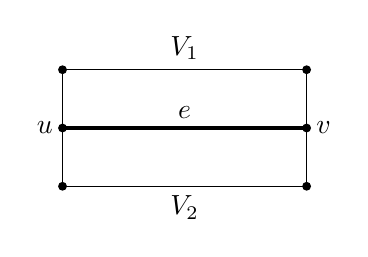
\begin{tikzpicture}[x=1cm,y=0.74cm]
\draw (-1.55,0)--(-1.55,1)--(1.55,1)--(1.55,0);
\draw (-1.55,0)--(-1.55,-1)--(1.55,-1)--(1.55,0);
\draw[very thick] (-1.55,0)--(1.55,0);
\foreach \x in {-1.55,1.55} \foreach \y in {-1,0,1}
  \fill (\x,\y) circle (1.6pt);
\node[left] at (-1.55,0) {\(u\)};
\node[right] at (1.55,0) {\(v\)};
\node[above] at (0,0) {\(e\)};
\node[above] at (0,1) {\(V_1\)};
\node[below] at (0,-1) {\(V_2\)};
\end{tikzpicture}

\small Two spatial faces. Their time evolution uses the same increment on \(e\).
\end{center}

\begin{theorem}\label{thm:isotropic-book}
Let \(G=\SU(2)\). On gauge-invariant states let \(\lambda_0(b)\) and
\(\lambda_1(b)\) be the two largest transfer eigenvalues, counted with
multiplicity. For every fixed \(m\ge1\),
\[
 \lim_{b\to\infty}\frac{\lambda_1(b)}{\lambda_0(b)}
 =
 \begin{cases}
 (3-2\sqrt2)^2,&m=1,\\[2pt]
 ((5-\sqrt{21})/2)^2,&m\ge2 .
 \end{cases}
\]
For each fixed \(m\), the supremum of this ratio over \(b\ge0\) is strictly
less than one. In particular one constant works for all four possible
cluster sizes \(1\le m\le4\) on the cubic spatial lattice.
\end{theorem}

\begin{proof}
Write \(U_0\) for the transporter along \(e\), \(V_i\) for the product along
private path \(i\), both oriented from \(u\) to \(v\), and \(P_i=V_iU_0^{-1}\).
Gauge fixing on a spanning tree leaves the \(m\) based loops up to
simultaneous conjugation. Equivalently, removing the interior vertices of
each path leaves only \(U_0,V_1,\ldots,V_m\), and setting \(U_0=I\)
leaves a single change of frame at \(u\). Under product Haar measure
the \(V_i\) are independent Haar variables independent of \(U_0\).
Conditioning on \(U_0\) shows that the \(P_i\) have product Haar law.
The physical Hilbert space is consequently the simultaneously invariant
subspace of \(L^2(G^m)\).

Put \(x(g)=\Tr(g)/2\), \(k_b(g)=e^{bx(g)}/\int_G e^{bx}\,dg\), with
probability Haar measure throughout. The free time step right multiplies
each link by an independent increment of density \(k_b\). On a serial
path, moving the increments to the end of the path conjugates them by
fixed products of old links. Centrality preserves their independent laws.
Inverting an oriented link gives the same law by inversion symmetry.
It follows that, conditional on the old configuration, the new loops have law
\[
 P'_i=P_i A_i W,\qquad
 A_1,\ldots,A_m\sim k_b^{*3},\quad W\sim k_b ,
\]
where the \(m+1\) variables are independent and \(W\) is common to every
face. Indeed \(U'_0=U_0 B_0\), \(V_i'=V_i B_i\), so the increments
in this formula are \(U_0B_iU_0^{-1}\) and \(U_0B_0^{-1}U_0^{-1}\).
If \(C\) denotes this transition and
\(D(P)=\exp[\frac b2\sum_i(x(P_i)-1)]\), the transfer up to a positive
scalar is \(DCD\). The kernel of \(C\) is
\[
 c_b(P,Q)=\int_G k_b(w)\prod_{i=1}^m
                 k_b^{*3}(P_i^{-1}Q_i w^{-1})\,dw .
\]
It is strictly positive. The transfer is positive semidefinite as well:
the central convolution on a link has eigenvalues
\(I_{\ell+1}(b)/I_1(b)>0\) for \(b>0\) in the irreducible representation
of dimension \(\ell+1\). This formula follows by integrating
\(e^{b\cos\theta}\sin((\ell+1)\theta)\sin\theta\) on \([0,\pi]\)
and integrating by parts. At \(b=0\) the transfer projects onto constants.
Passing to the physical subspace preserves positivity.

\smallskip\noindent\emph{The weak-coupling limit.}
In unit-quaternion coordinates let
\(g_y=(\cos t,\widehat y\sin t)\), \(t=|y|/\sqrt b\), for
\(|y|<\pi\sqrt b\). The Haar density with respect to \(dy\) is
\(J_b(y)=j_b(\sin t/t)^2\), \(j_b=(2\pi^2 b^{3/2})^{-1}\).
Multiplication by \(J_b^{1/2}\) in these coordinates and extension by zero
embed each copy of \(L^2(G)\) isometrically in \(L^2(\R^3)\).
Since \(1-\cos t\ge2t^2/\pi^2\), dominated convergence in the normalizing
integral gives \(j_b k_b(g_y)\to(2\pi)^{-3/2}e^{-|y|^2/2}\).
Moreover \(j_b\|k_b\|_\infty\) is bounded for \(b\ge1\), and
\(J_b(y)k_b(g_y)\le C_0 e^{-2|y|^2/\pi^2}\) with an absolute \(C_0\).

For a fixed scaled argument \(s\), the density
\(j_b k_b^{*3}(g_s)\) converges to the density of a centered normal
variable of covariance \(3I_3\), also along any \(s_b\to s\).
To see this, write the convolution using two independent increments and the
density of the third. The first two scaled increments have the Gaussian
majorant above. The last density times \(j_b\) is uniformly bounded.
For fixed scaled inputs, quaternion multiplication adds their vector parts
to first order in \(b^{-1/2}\), with error \(O(b^{-1})\) before rescaling.
Dominated convergence gives precisely the convolution of three standard
Gaussian densities. Applying the same argument to the \(w\)-integral for
\(c_b\) gives a joint normal density for the displacement from \(y\) to \(z\)
with covariance \(\Sigma\otimes I_3\), where
\[
 \Sigma=3I_m+\mathbf 1\mathbf 1^{\mathsf T}.
\]
In particular the common increment contributes an off-diagonal covariance
of one. The two factors \(D\) converge to \(e^{-|y|^2/4}\) and
\(e^{-|z|^2/4}\). For each fixed \(m\) the transformed transfer kernels are
bounded by \(C_m\exp[-(|y|^2+|z|^2)/\pi^2]\), since
\(\|k_b^{*3}\|_\infty\le\|k_b\|_\infty\) and \(J_b\le j_b\).
The square of the bound is integrable. The kernels therefore converge in
Hilbert--Schmidt norm. Simultaneous conjugation acts as the same spatial
rotation on every three-vector, so restriction to its invariant subspace
commutes with this convergence.

\smallskip\noindent\emph{The first invariant excitation.}
Diagonalizing \(\Sigma\) mixes the face indices and preserves the rotation
action. A coordinate with variance \(v\) has Gaussian kernel proportional to
\[
 e^{-A(y^2+z^2)+B yz},\qquad A=\tfrac14+\tfrac1{2v},\quad B=\tfrac1v.
\]
Its ground state is \(e^{-\gamma y^2}\),
\(\gamma=(A^2-B^2/4)^{1/2}\). Completing the square in the \(z\) integral
shows that a polynomial of degree \(d\) times the ground state is mapped
to a polynomial of degree at most \(d\) times that state. Its top coefficient
is multiplied by the ground eigenvalue times
\[
 r(v)^d,\qquad
 r(v)=\frac{B}{2(A+\gamma)}
     =\frac{2}{2+v+\sqrt{v(v+4)}} .
\]
Orthogonalizing by degree diagonalizes these nested polynomial spaces,
whose Gaussian-weighted union is dense by the Hermite expansion.
Tensor products give the full spectrum in all modes. The ground state is a
rotation scalar. A degree-one excitation transforms as a vector, so none is
invariant. The square norm of any three-vector mode, centered against the
squared ground state, supplies an invariant excitation of degree two.
Consequently the first invariant eigenvalue ratio is \(r(v_{\min})^2\):
all excitations of degree at least two have ratio at most this large.
For one face the variance is four. For \(m\ge2\) the difference modes
have variance three and the common mode has variance \(3+m\).
The min--max principle and the norm convergence now give the stated limits.

At finite \(b\) the continuous strictly positive kernel on compact \(G^m\)
has a simple largest eigenvalue and a strictly positive ground state, which
is invariant by uniqueness. Indeed, replacing a sign-changing maximizer
by its absolute value strictly increases its quadratic form, and two
orthogonal ground states cannot both have constant sign. The kernels are
continuous in \(b\) in operator norm on every compact interval. Compactness
therefore bounds the ratio strictly below one on each such interval.
The limit at infinity supplies the remaining uniformity for fixed \(m\).
\end{proof}

\subsection*{A cube with all its spatial plaquettes}
Now take the cubic grid \(\{0,\ldots,L\}^3\), with every elementary
spatial plaquette present and free spatial boundary. We impose the Gauss
constraint at every vertex, including the boundary. The integer \(L\)
counts intervals along one side. Write \(\Delta_L(b)=
-\log(\lambda_1(b)/\lambda_0(b))\) for the gauge-invariant gap in lattice
time units.

\begin{theorem}\label{thm:isotropic-free-box}
For equal spatial and temporal Wilson couplings in \(\SU(2)\),
\[
 \lim_{b\to\infty}\Delta_L(b)
    =4\operatorname{arsinh}\!\left(\sqrt2\sin\frac{\pi}{2(L+1)}\right)
 \qquad (L\ge1\text{ fixed}).
\]
In particular \(\inf_{b>0}\Delta_L(b)>0\) for each fixed \(L\).
The displayed limit is asymptotic to \(2\sqrt2\,\pi/(L+1)\) as
\(L\to\infty\).
\end{theorem}

\begin{proof}
Orient the edges, choose a rooted spanning tree, and write \(s\) for the
number of edges outside the tree. After gauge fixing there are \(s\) based
holonomies \(P_e\) with product Haar measure, modulo one simultaneous
conjugation. In fact, conditional on the old tree links, each chord link
is independent Haar; left and right multiplication by the two endpoint
transporters preserves that conditional law. Take the representative with
all tree links equal to \(I\). Let \(V(P)=\sum_f(1-x(U_f(P)))\), the sum
over all elementary faces in this representative. If \(V=0\), each face
has identity holonomy. Every edge loop in this box contracts by elementary
face moves and backtracking, so every \(P_e=I\).

Let \(d_0,d_1\) be the vertex-to-edge difference and edge-to-face curl
on real cochains with orthonormal cell bases. Let \(B\) send an edge
vector to the signed sums along the rooted fundamental cycles. Let \(S\)
extend a chord vector by zero on the tree. Then \(BS=I_s\) and
\(a-SBa\) is a gradient: integrating \(a\) along the tree determines its
vertex potential, and the zero fundamental cycle sums determine the
chord differences. Setting \(F=d_1 S\) gives \(d_1=FB\).
The matrix \(F\) is injective since a curl-free edge vector on the box is
a gradient, and a gradient vanishing on the tree vanishes everywhere.
In local quaternion coordinates \(P_e=\exp y_e\), with
\(\exp y=(\cos|y|,\widehat y\sin|y|)\), the plaquette products give
\[
 V(P)=\tfrac12\sum_f\left|\sum_e F_{fe}y_e\right|^2+O_L(|y|^3).
\]
Injectivity gives a positive local quadratic lower bound. By compactness
and the unique zero proved above, for some \(c_L>0\) we have globally
\[
 V(P)\ge c_L\sum_e \operatorname{dist}(P_e,I)^2
\]
in unit-sphere geodesic distance. This is the place where free boundary
and simple connectivity enter the estimate.\footnote{On a spatial torus,
constant commuting links can have nontrivial holonomy around a periodic
direction while every plaquette has identity holonomy. The stated global
inequality in based chord coordinates then fails.}

For clarity, integrate one exact time step in the tree gauge. Let \(W_t\)
be the new increments on tree links and let \(T_v\) be their oriented
product on the tree path from the root to \(v\). For a chord \(e=(u,v)\),
the new based holonomy is \(Q_e=T_u P_e W_e T_v^{-1}\). Conditional on
the tree increments the \(W_e\) of the chords are independent. Thus the
transition kernel is the average over \(W_t\) of
\[
 \prod_{e=(u,v)\ {\rm chord}} k_b(P_e^{-1}T_u^{-1}Q_e T_v).
\]
It is bounded by \(\|k_b\|_\infty^s\). At \(P_e=g_{y_e}\),
\(Q_e=g_{z_e}\), each tree increment, rescaled by \(\sqrt b\), has the
integrable Gaussian majorant used in Theorem~\ref{thm:isotropic-book}.
The chord density factors, each multiplied by \(j_b\), are bounded
uniformly. Linearizing the path products at fixed scaled increments shows
that the rescaled displacement is \(B\) applied to independent standard
three-dimensional normal increments on \emph{all} edges. Equivalently the
conditional limit is a product of unit-variance chord densities shifted
by the signed tree sums, integrated against the independent tree Gaussians.
Dominated convergence therefore gives the joint normal density with
covariance \(\Sigma\otimes I_3\), \(\Sigma=BB^{\mathsf T}>0\).

With the square roots of the Haar Jacobians included, the symmetric
transfer is bounded by \(C_L e^{-c_L(|y|^2+|z|^2)/2}\), by the global
estimate for \(V\). Its limit is the normal transition just derived
multiplied on each side by
\(\exp[-\sum_f|\sum_e F_{fe} y_e|^2/4]\) in the corresponding variable.
The convergence is Hilbert--Schmidt for fixed \(L\); in particular it
holds after projection on the simultaneous rotation invariants. Whitening
the covariance by \(y=\Sigma^{1/2}u\) leaves unit kinetic variance and
potential matrix \(\Sigma^{1/2}F^{\mathsf T}F\Sigma^{1/2}\), with the
same matrix in each color. Its eigenvalues are the positive eigenvalues
of \(d_1^{\mathsf T}d_1\), since \(F\Sigma F^{\mathsf T}
=d_1d_1^{\mathsf T}\). A mode of potential strength \(\kappa>0\) and
unit kinetic variance has level ratio \(r(\kappa)\), by the preceding
Gaussian calculation after rescaling that mode. Thus its level spacing is
\(2\operatorname{arsinh}(\sqrt\kappa/2)\). Again the first invariant
excitation is quadratic in a lowest three-vector mode and has twice that
spacing. Positivity and continuity at finite \(b\) give the strict lower
bound for fixed \(L\) as in Theorem~\ref{thm:isotropic-book}.

It remains to evaluate the smallest positive curl eigenvalue with these
boundary conditions. The one-dimensional difference from \(L+1\) vertices
to \(L\) edges has singular values
\[
 d_j=2\sin\frac{\pi j}{2(L+1)},\quad 1\le j\le L .
\]
Indeed its product with its transpose is the \(L\)-by-\(L\) tridiagonal
matrix with diagonal two and off-diagonals minus one; the sine vectors
diagonalize it. The additional vertex mode \(j=0\) is constant and has
\(d_0=0\) in this scalar notation. In the tensor product of the three
one-dimensional singular bases, fix indices \(j_1,j_2,j_3\) and write
\(d=(d_{j_1},d_{j_2},d_{j_3})\). The edge cochain has one component
for each nonzero index, since a zero index has no edge vector.
Its gradient direction is \(d\) and the curl is \(a\mapsto d\wedge a\)
by the oriented face difference formula. The identity
\(\|d\wedge a\|^2=|d|^2|a|^2-|d\cdot a|^2\) shows that a positive
eigenvalue requires at least two nonzero indices, and then equals
\(|d|^2\) on the orthogonal complement of \(d\). The minimum is
\(2d_1^2=8\sin^2(\pi/(2(L+1)))\), attained at \((1,1,0)\).
Substitution and the small-argument expansion of sine and inverse
hyperbolic sine give both formulas.
\end{proof}

The deterioration in \(L\) is explicit. The theorem first sends the bare
coupling parameter \(b\) to infinity on a fixed free box. Along a continuum
trajectory, the number of lattice intervals in a fixed physical length
grows while the coupling changes. Controlling the errors in that joint
limit, the periodic holonomies, and the resulting infinite-volume theory
requires estimates beyond this fixed-box spectrum.

\subsection*{What an omitted face contributes}
There is an obstruction to replacing a cubic lattice by independent spatial
plaquettes. Take a periodic spatial lattice of side at least four and a
time circle of \(h\ge2\) steps. In temporal gauge consider the ordinary
periodic trace before the projection onto gauge-invariant states.
Retain the full Wilson weight at coupling \(b\) on an edge-disjoint set
of spatial plaquettes and omit the other spatial weights. Write \(\E_0\)
for this probability law. For an omitted face \(p\), put
\(S=\sum_{j=0}^{h-1}x_p(j)\). Then
\[
 A_h=\E_0 e^{bS}\ \ge\ 1+b^2h/8,\qquad
 \E_0\big[(e^{bS}/A_h-1)^2\big]\ \ge\ 1-A_h^{-2}.
\]
Indeed, the kinetic term couples only successive copies of the same link.
The reference measure factors over the retained squares and the remaining
individual link histories. At any fixed time, each individual link of a
retained square is Haar: time-independent changes of frame at an endpoint
preserve that factor and act transitively on the link. Distinct elementary
faces share at most one edge, so the four links of \(p\) belong to different
factors. Their product is Haar and \(\E_0 x_p(j)^2=1/4\), by the second
coordinate moment of the uniform unit three-sphere. Multiplying one link
history of \(p\) by \(-I\) reverses \(S\). If that link belongs to a retained
square, multiply a second link of that square by \(-I\) as well. This leaves
the reference law invariant, so \(S\) has a symmetric distribution.
For its positive transfer operator \(K\) and multiplication \(M\) by \(x_p\),
the numerator of the lag-\(j\) correlation is \(\Tr(MK^jMK^{h-j})\).
It is the squared Hilbert--Schmidt norm of
\(K^{j/2} M K^{(h-j)/2}\). Hence \(\E_0 S^2\ge h/4\). Now
\(A_h=\E_0\cosh(bS)\ge1+b^2\E_0 S^2/2\), and
\(\E_0e^{2bS}=2\E_0\cosh^2(bS)-1\ge2A_h^2-1\), proving both bounds.

The theorem treats overlapping faces around one link with free boundary.
In a cubic lattice a face also interacts through its other three links.
The lower bound above shows why a small-activity expansion about
edge-disjoint faces loses control at equal large couplings. The transfer
estimate on a cube of fixed physical size still requires control of the
joint law of all those overlaps as the lattice spacing tends to zero.
